\chapter{Описание численного алгоритма решения} \label{ch2}

Совмещение формулы Кёнинга с уравнениями Кирхгофа проводится следующим образом:

1) на текущем шаге по времени по имеющимся значениям полудлины трещин автоГРП предыдущего шага рассчитываются давления и расходы на каждой трещине;

2) на основе полученных значений приращений давления и расхода рассчитывается приращение полудлины трещины $dx_{\!f}$ на данном временном шаге по формуле \eqref{IncrementExplicit_first} в случае одномерных утечек Картера и по формуле \eqref{IncrementExplicit_second} в случае двумерных радиальных утечек жидкости из трещины в пласт;

3) по формуле $x_{\!f}^{\text{current}}=x_{\!f}^{\text{last}}+dx_{\!f}$ рассчитываются полудлины каждой из трещин на текущем временном шаге;

4) описанные действия повторяются до требуемого шага по времени (условия остановки).

На рис. \ref{fig:koning_scheme} этот алгоритм расчёта полудлин растущих трещин автоГРП представлен в виде блок-схемы.

\begin{figure}[H] 
\center
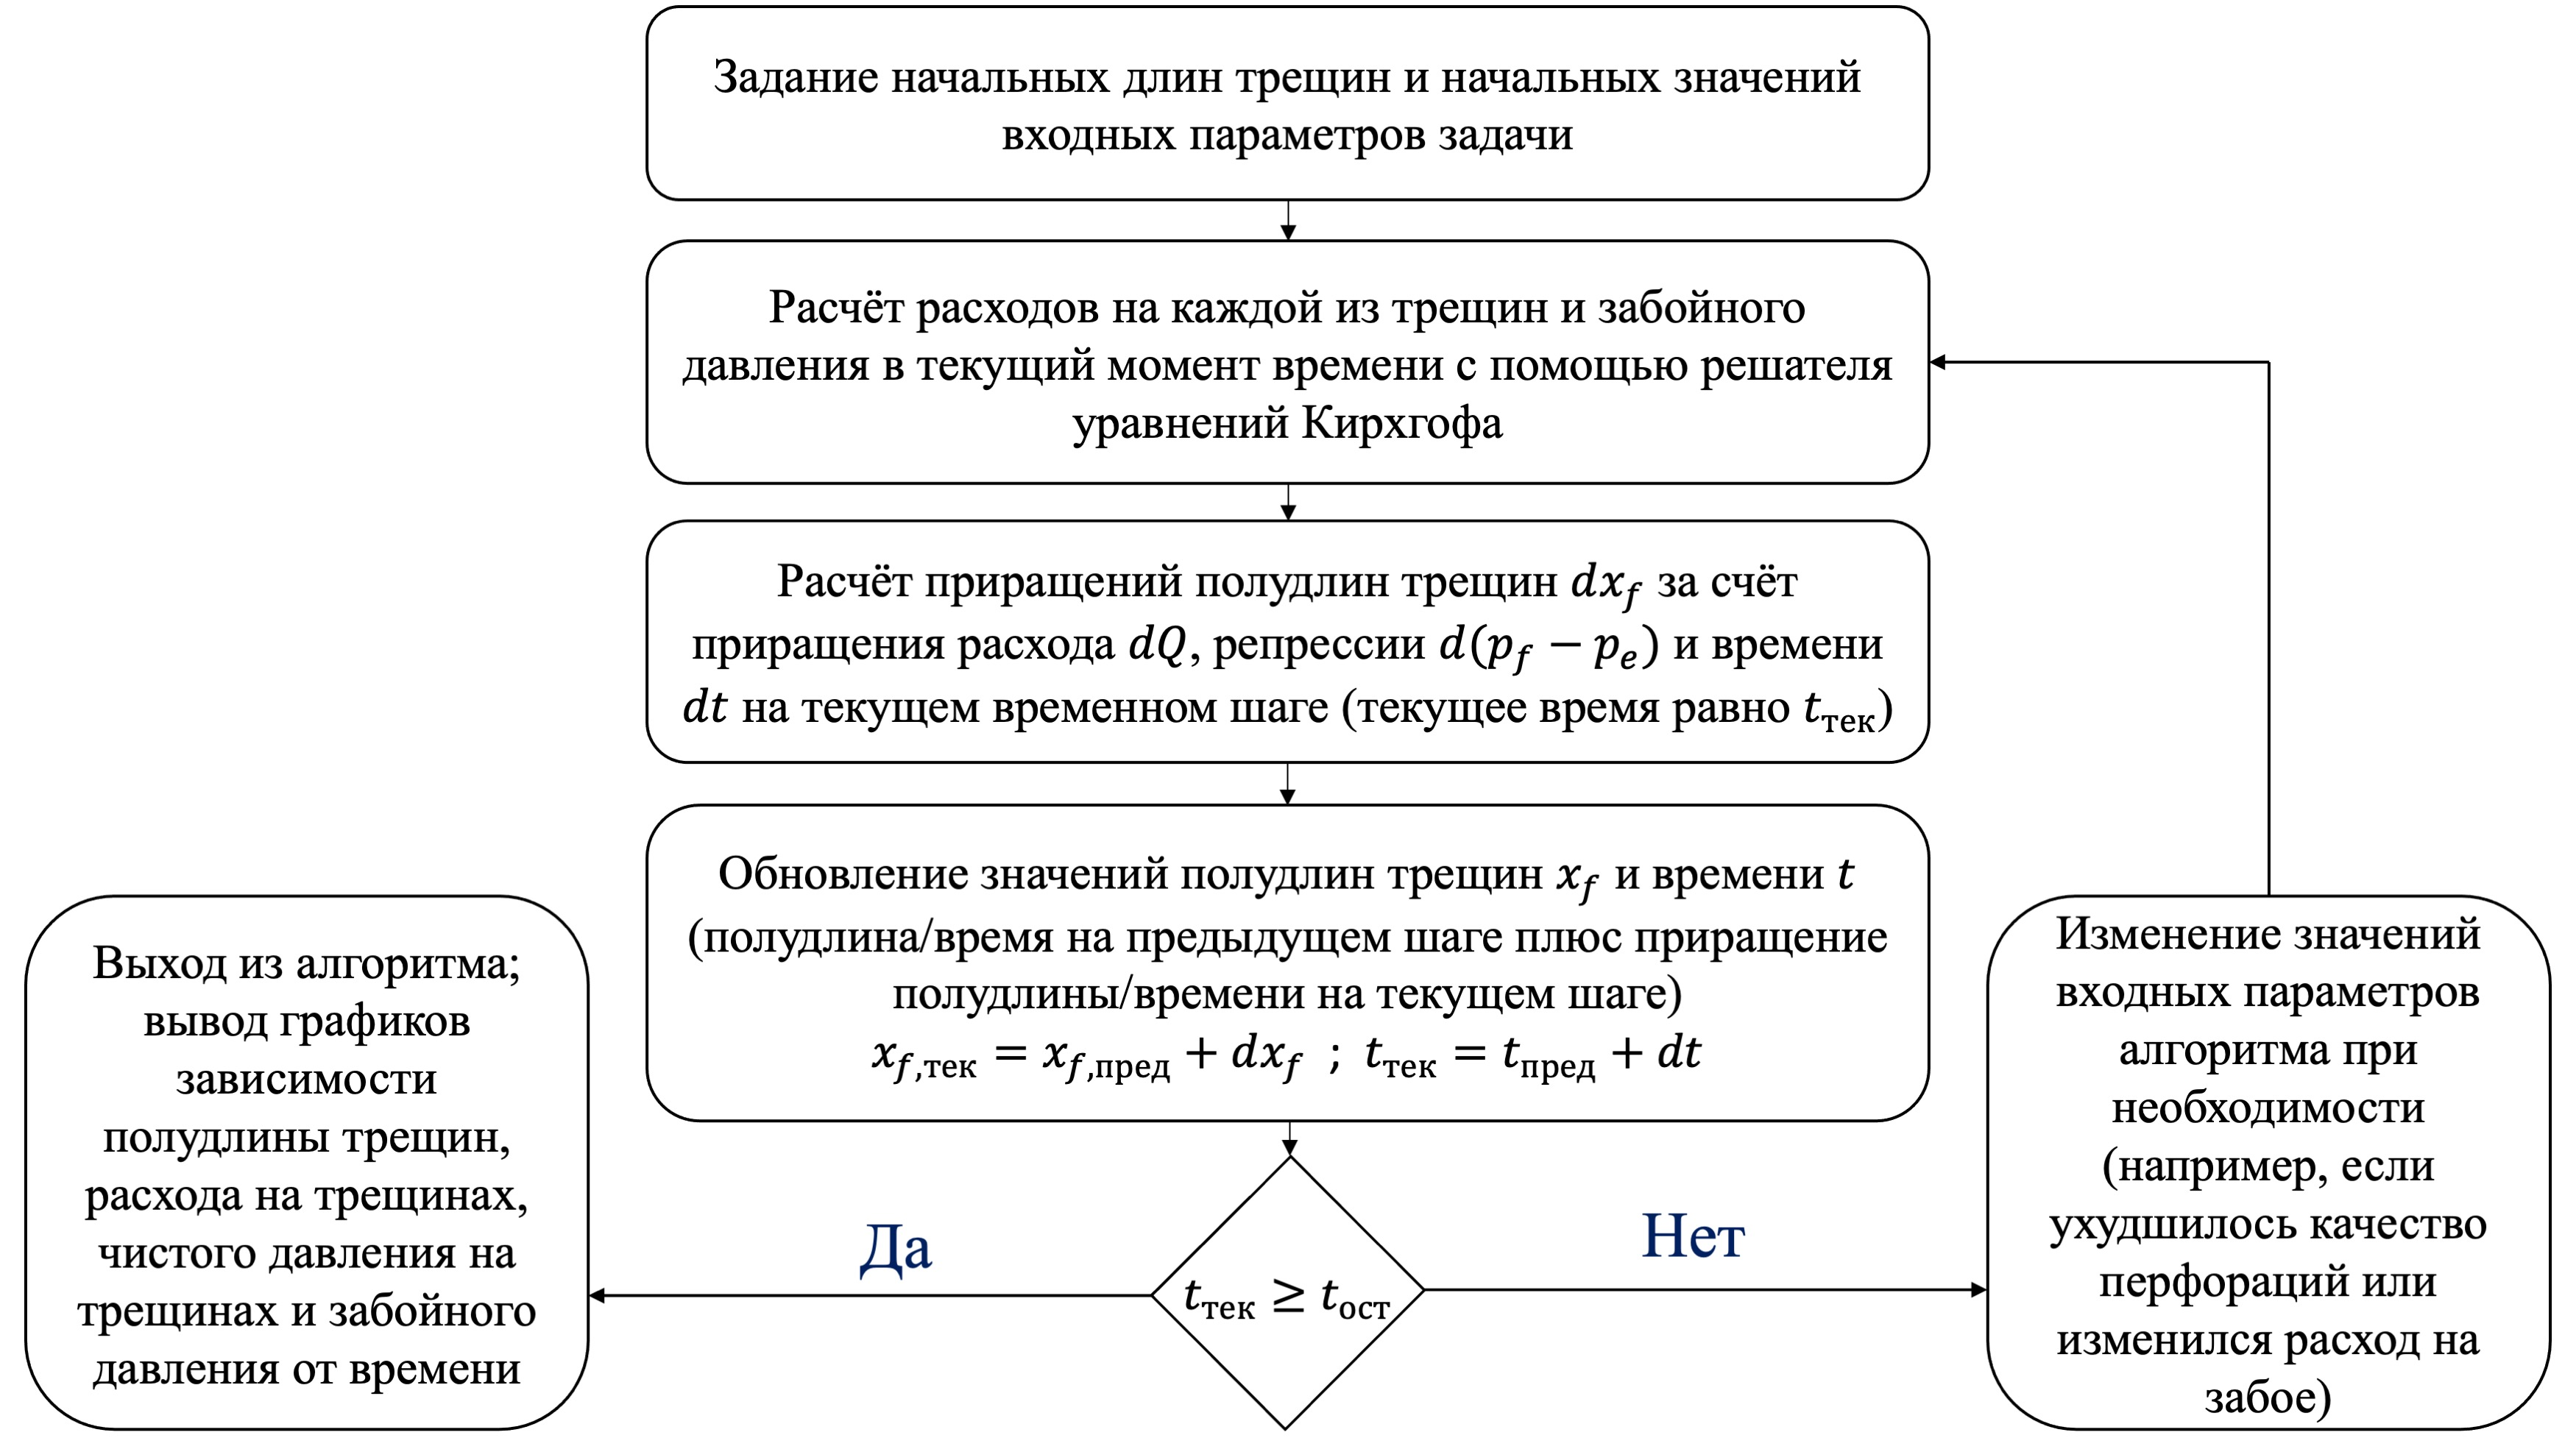
\includegraphics[width=\linewidth]{images/Koning_scheme.jpg}
\caption{Алгоритм расчёта полудлин трещин в зависимости от времени} 
\label{fig:koning_scheme}
\end{figure}




